\documentclass[11pt]{article}
\usepackage[textwidth=18.0cm, textheight=23.0cm, top=2.0cm]{geometry}
\usepackage{pst-all}
\usepackage{amssymb}
\usepackage{tikz}
\usepackage{underscore}\begin{document}
\pagestyle{empty}


ClassName: \underline{\textbf{Class_05.2bp-13}}
\par
BinSize: \underline{\textbf{100 × 100}}
\par
ReduceSize: \underline{\textbf{100 × 100}}
\par
TypeNum: \underline{\textbf{40}}
\par
Num: \underline{\textbf{40}}
\par
OutS: \underline{\textbf{130000}}
\par
InS: \underline{\textbf{104282}}
\par
Rate: \underline{\textbf{0.802}}
\par
UB: \underline{\textbf{13}}
\par
LB0: \underline{\textbf{12}}
\par
LB: \underline{\textbf{13}}
\par
LBWithCut: \underline{\textbf{13}}
\par
NodeCut: \underline{\textbf{0}}
\par
ExtendedNodeCnt: \underline{\textbf{1}}
\par
GenNodeCnt: \underline{\textbf{1}}
\par
PrimalNode: \underline{\textbf{0}}
\par
ColumnCount: \underline{\textbf{75}}
\par
TotalCutCount: \underline{\textbf{0}}
\par
RootCutCount: \underline{\textbf{0}}
\par
LPSolverCnt: \underline{\textbf{63}}
\par
PricingSolverCnt: \underline{\textbf{63}}
\par
BranchAndBoundNum: \underline{\textbf{1}}
\par
isOpt: \underline{\textbf{true}}
\par
TimeOnInitSolution: \underline{\textbf{600.000 s}}
\par
TimeOnPrimal: \underline{\textbf{0.000 s}}
\par
TimeOnPricing: \underline{\textbf{17.645 s}}
\par
TimeOnRmp: \underline{\textbf{0.122 s}}
\par
TotalTime: \underline{\textbf{618.050 s}}
\par
\newpage


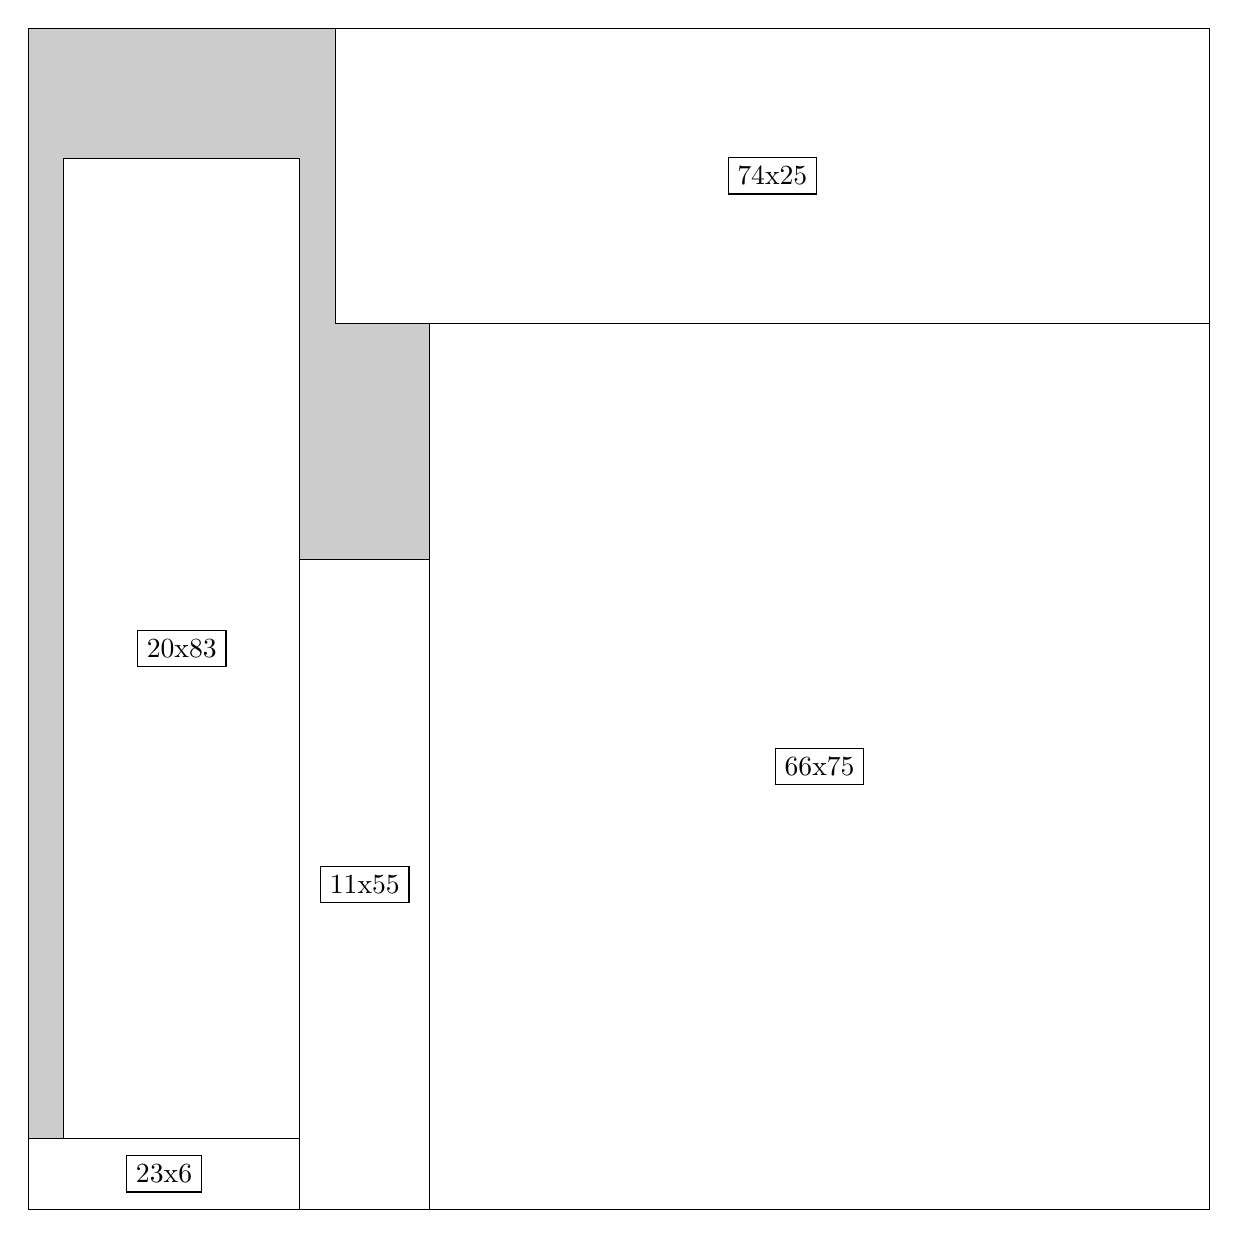
\begin{tikzpicture}[shorten >=1pt,scale=1.0,every node/.style={scale=1.0},->]
\tikzstyle{vertex}=[circle,fill=black!25,minimum size=14pt,inner sep=0pt]
\filldraw[fill=gray!40!white, draw=black] (0,0) rectangle (15.0,15.0);
\foreach \name/\x/\y/\w/\h in {66x75/5.1/0.0/9.9/11.25,11x55/3.4499999999999997/0.0/1.65/8.25,74x25/3.9/11.25/11.1/3.75,23x6/0.0/0.0/3.4499999999999997/0.8999999999999999,20x83/0.44999999999999996/0.8999999999999999/3.0/12.45}
\filldraw[fill=white!40!white, draw=black] (\x,\y) rectangle node[draw] (\name) {\name} ++(\w,\h);
\end{tikzpicture}


w =66 , h =75 , x =34 , y =0 , v =4950
\par
w =11 , h =55 , x =23 , y =0 , v =605
\par
w =74 , h =25 , x =26 , y =75 , v =1850
\par
w =23 , h =6 , x =0 , y =0 , v =138
\par
w =20 , h =83 , x =3 , y =6 , v =1660
\par
\newpage


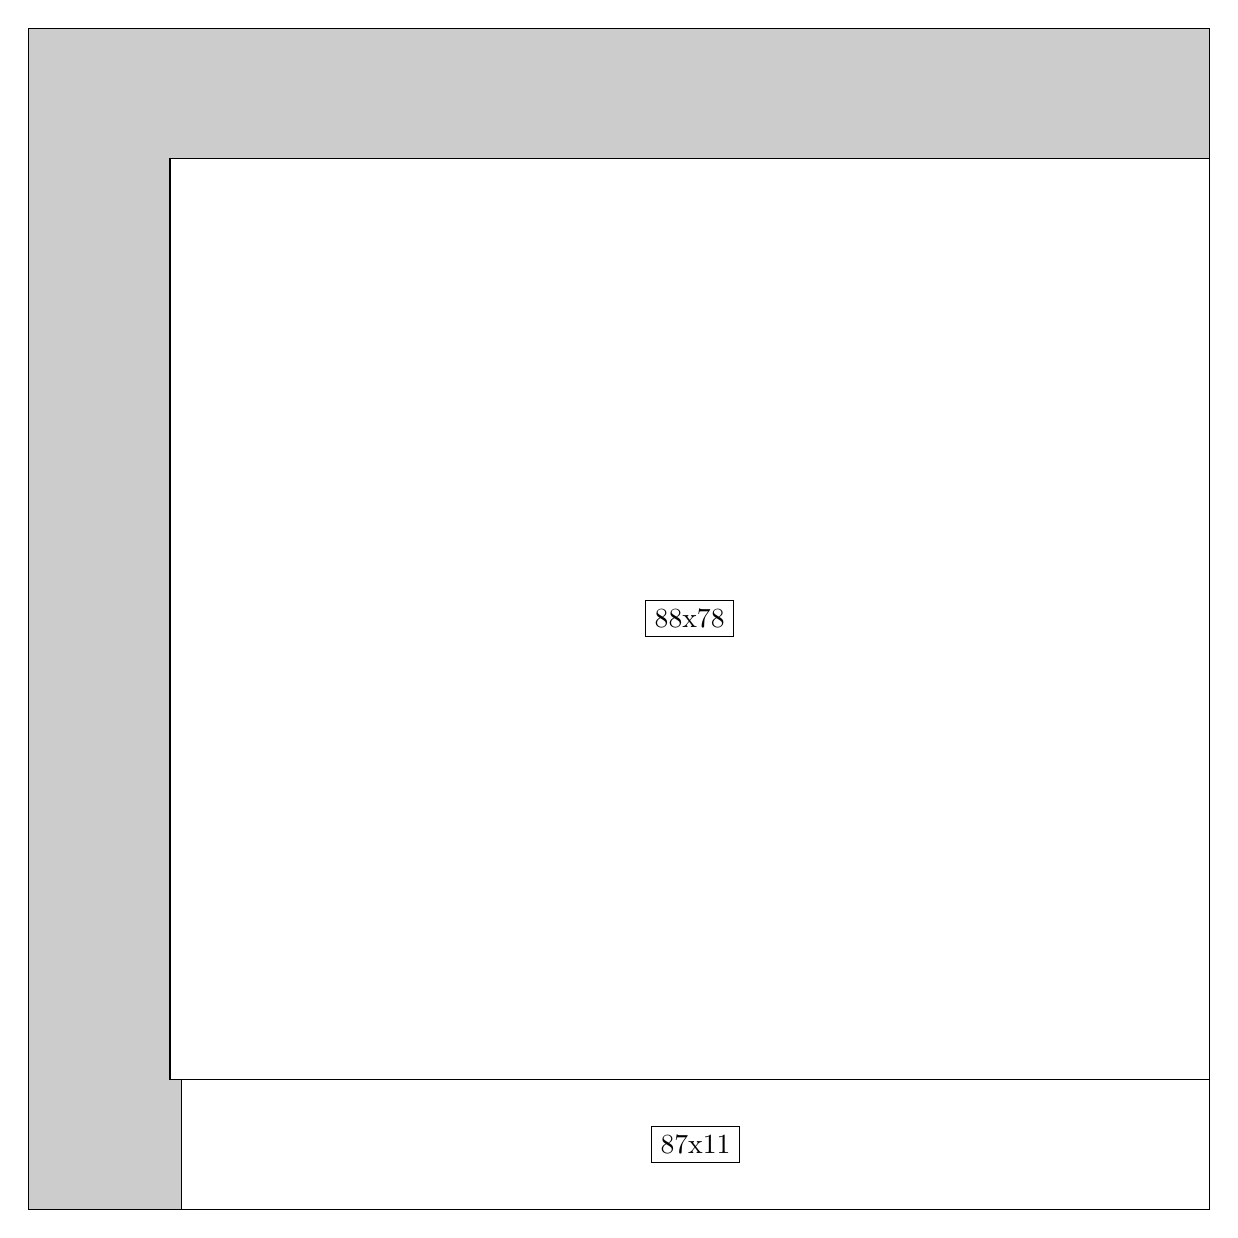
\begin{tikzpicture}[shorten >=1pt,scale=1.0,every node/.style={scale=1.0},->]
\tikzstyle{vertex}=[circle,fill=black!25,minimum size=14pt,inner sep=0pt]
\filldraw[fill=gray!40!white, draw=black] (0,0) rectangle (15.0,15.0);
\foreach \name/\x/\y/\w/\h in {87x11/1.95/0.0/13.049999999999999/1.65,88x78/1.7999999999999998/1.65/13.2/11.7}
\filldraw[fill=white!40!white, draw=black] (\x,\y) rectangle node[draw] (\name) {\name} ++(\w,\h);
\end{tikzpicture}


w =87 , h =11 , x =13 , y =0 , v =957
\par
w =88 , h =78 , x =12 , y =11 , v =6864
\par
\newpage


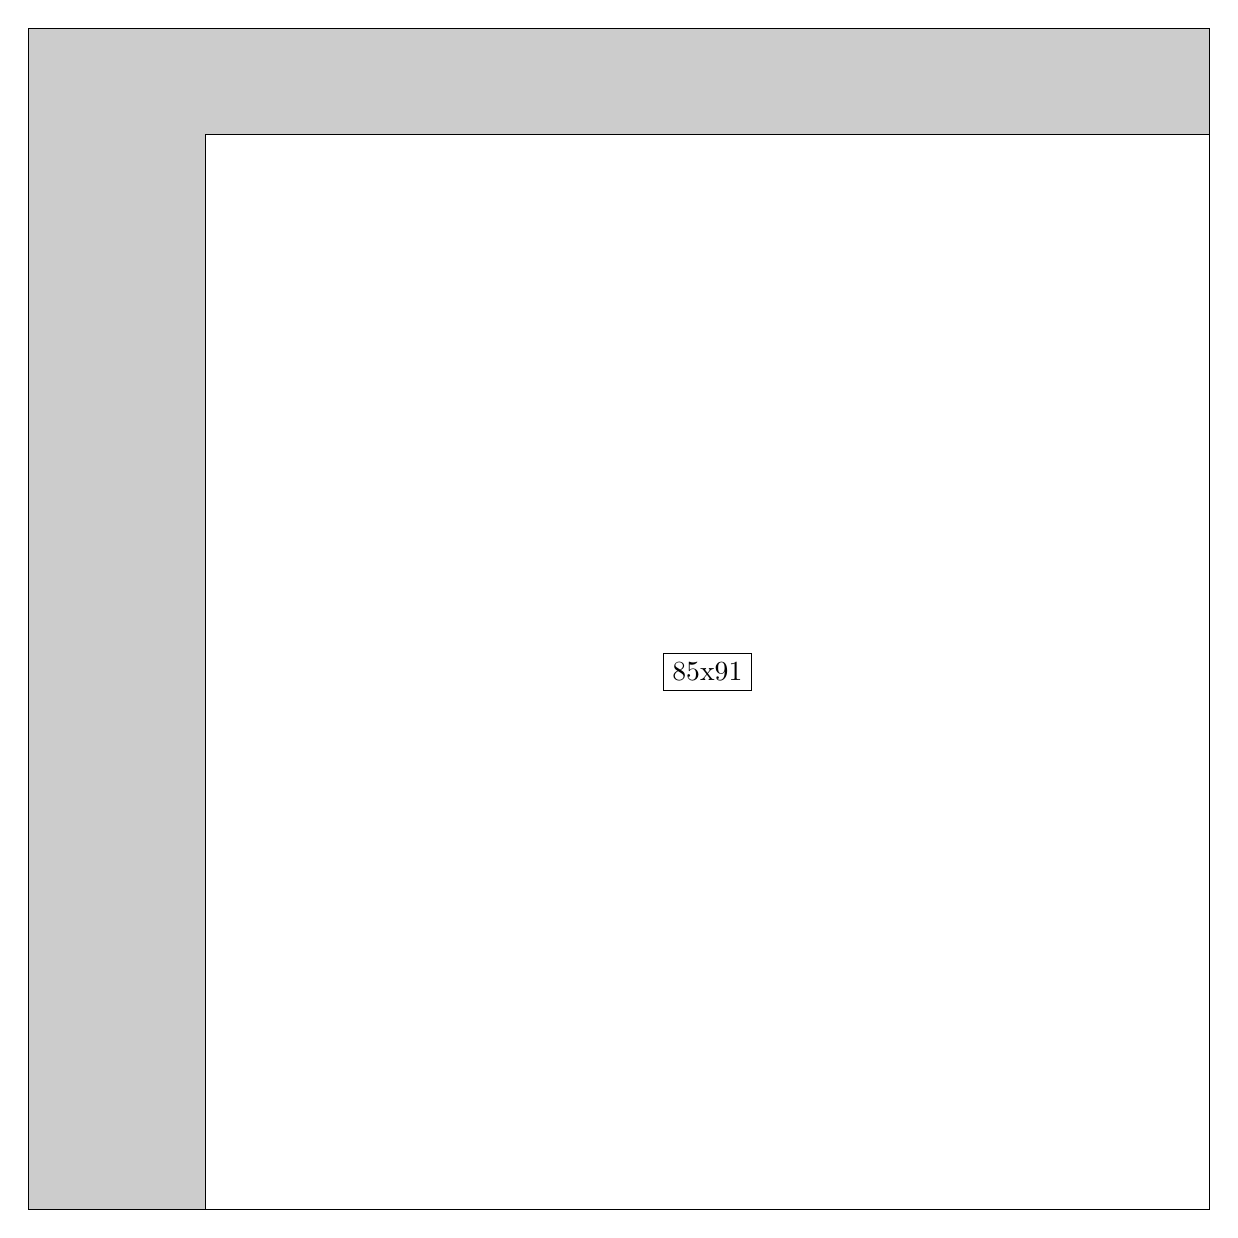
\begin{tikzpicture}[shorten >=1pt,scale=1.0,every node/.style={scale=1.0},->]
\tikzstyle{vertex}=[circle,fill=black!25,minimum size=14pt,inner sep=0pt]
\filldraw[fill=gray!40!white, draw=black] (0,0) rectangle (15.0,15.0);
\foreach \name/\x/\y/\w/\h in {85x91/2.25/0.0/12.75/13.65}
\filldraw[fill=white!40!white, draw=black] (\x,\y) rectangle node[draw] (\name) {\name} ++(\w,\h);
\end{tikzpicture}


w =85 , h =91 , x =15 , y =0 , v =7735
\par
\newpage



\begin{tikzpicture}[shorten >=1pt,scale=1.0,every node/.style={scale=1.0},->]
\tikzstyle{vertex}=[circle,fill=black!25,minimum size=14pt,inner sep=0pt]
\filldraw[fill=gray!40!white, draw=black] (0,0) rectangle (15.0,15.0);
\foreach \name/\x/\y/\w/\h in {96x93/0.6/0.0/14.399999999999999/13.95}
\filldraw[fill=white!40!white, draw=black] (\x,\y) rectangle node[draw] (\name) {\name} ++(\w,\h);
\end{tikzpicture}


w =96 , h =93 , x =4 , y =0 , v =8928
\par
\newpage


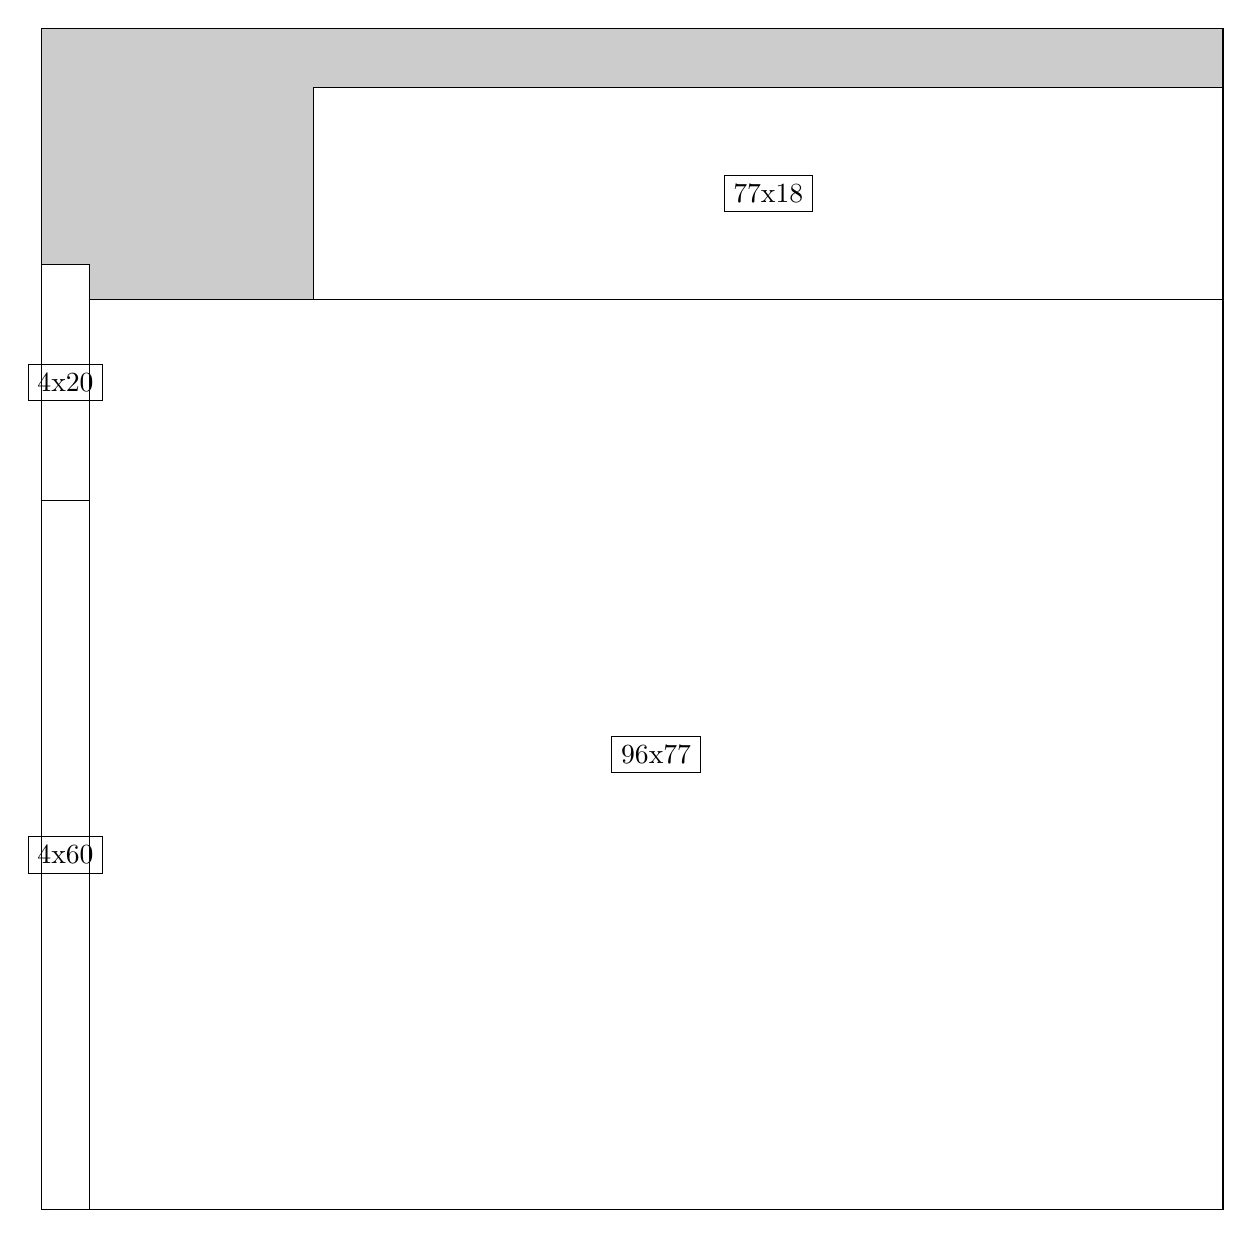
\begin{tikzpicture}[shorten >=1pt,scale=1.0,every node/.style={scale=1.0},->]
\tikzstyle{vertex}=[circle,fill=black!25,minimum size=14pt,inner sep=0pt]
\filldraw[fill=gray!40!white, draw=black] (0,0) rectangle (15.0,15.0);
\foreach \name/\x/\y/\w/\h in {96x77/0.6/0.0/14.399999999999999/11.549999999999999,77x18/3.4499999999999997/11.549999999999999/11.549999999999999/2.6999999999999997,4x60/0.0/0.0/0.6/9.0,4x20/0.0/9.0/0.6/3.0}
\filldraw[fill=white!40!white, draw=black] (\x,\y) rectangle node[draw] (\name) {\name} ++(\w,\h);
\end{tikzpicture}


w =96 , h =77 , x =4 , y =0 , v =7392
\par
w =77 , h =18 , x =23 , y =77 , v =1386
\par
w =4 , h =60 , x =0 , y =0 , v =240
\par
w =4 , h =20 , x =0 , y =60 , v =80
\par
\newpage


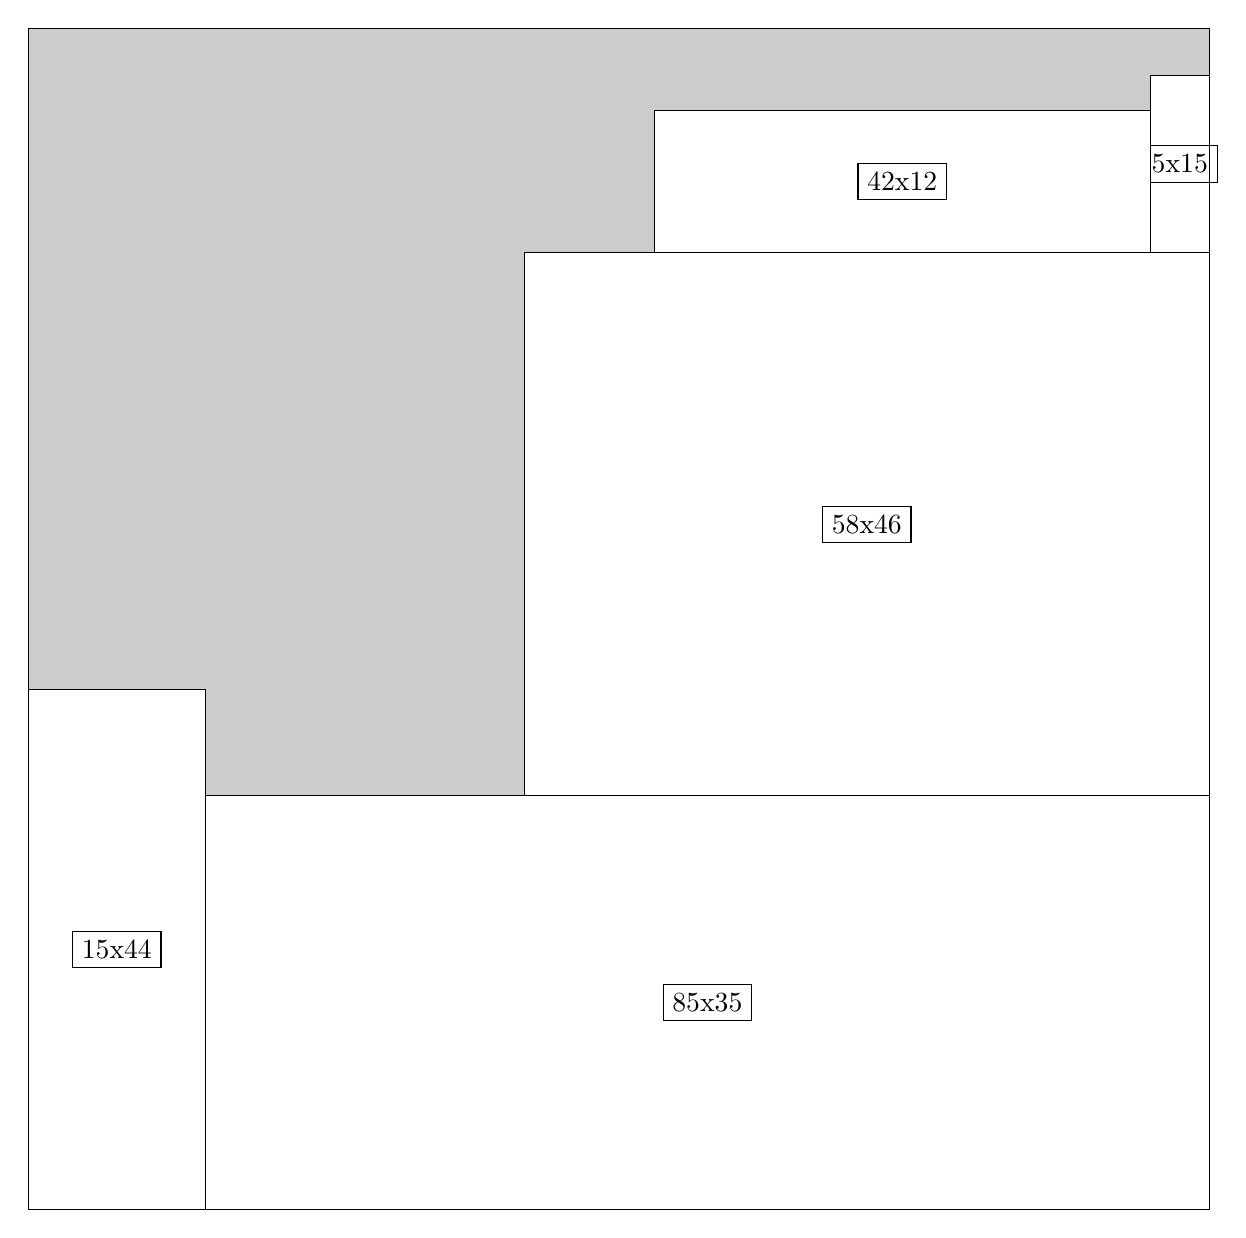
\begin{tikzpicture}[shorten >=1pt,scale=1.0,every node/.style={scale=1.0},->]
\tikzstyle{vertex}=[circle,fill=black!25,minimum size=14pt,inner sep=0pt]
\filldraw[fill=gray!40!white, draw=black] (0,0) rectangle (15.0,15.0);
\foreach \name/\x/\y/\w/\h in {85x35/2.25/0.0/12.75/5.25,58x46/6.3/5.25/8.7/6.8999999999999995,5x15/14.25/12.15/0.75/2.25,42x12/7.949999999999999/12.15/6.3/1.7999999999999998,15x44/0.0/0.0/2.25/6.6}
\filldraw[fill=white!40!white, draw=black] (\x,\y) rectangle node[draw] (\name) {\name} ++(\w,\h);
\end{tikzpicture}


w =85 , h =35 , x =15 , y =0 , v =2975
\par
w =58 , h =46 , x =42 , y =35 , v =2668
\par
w =5 , h =15 , x =95 , y =81 , v =75
\par
w =42 , h =12 , x =53 , y =81 , v =504
\par
w =15 , h =44 , x =0 , y =0 , v =660
\par
\newpage


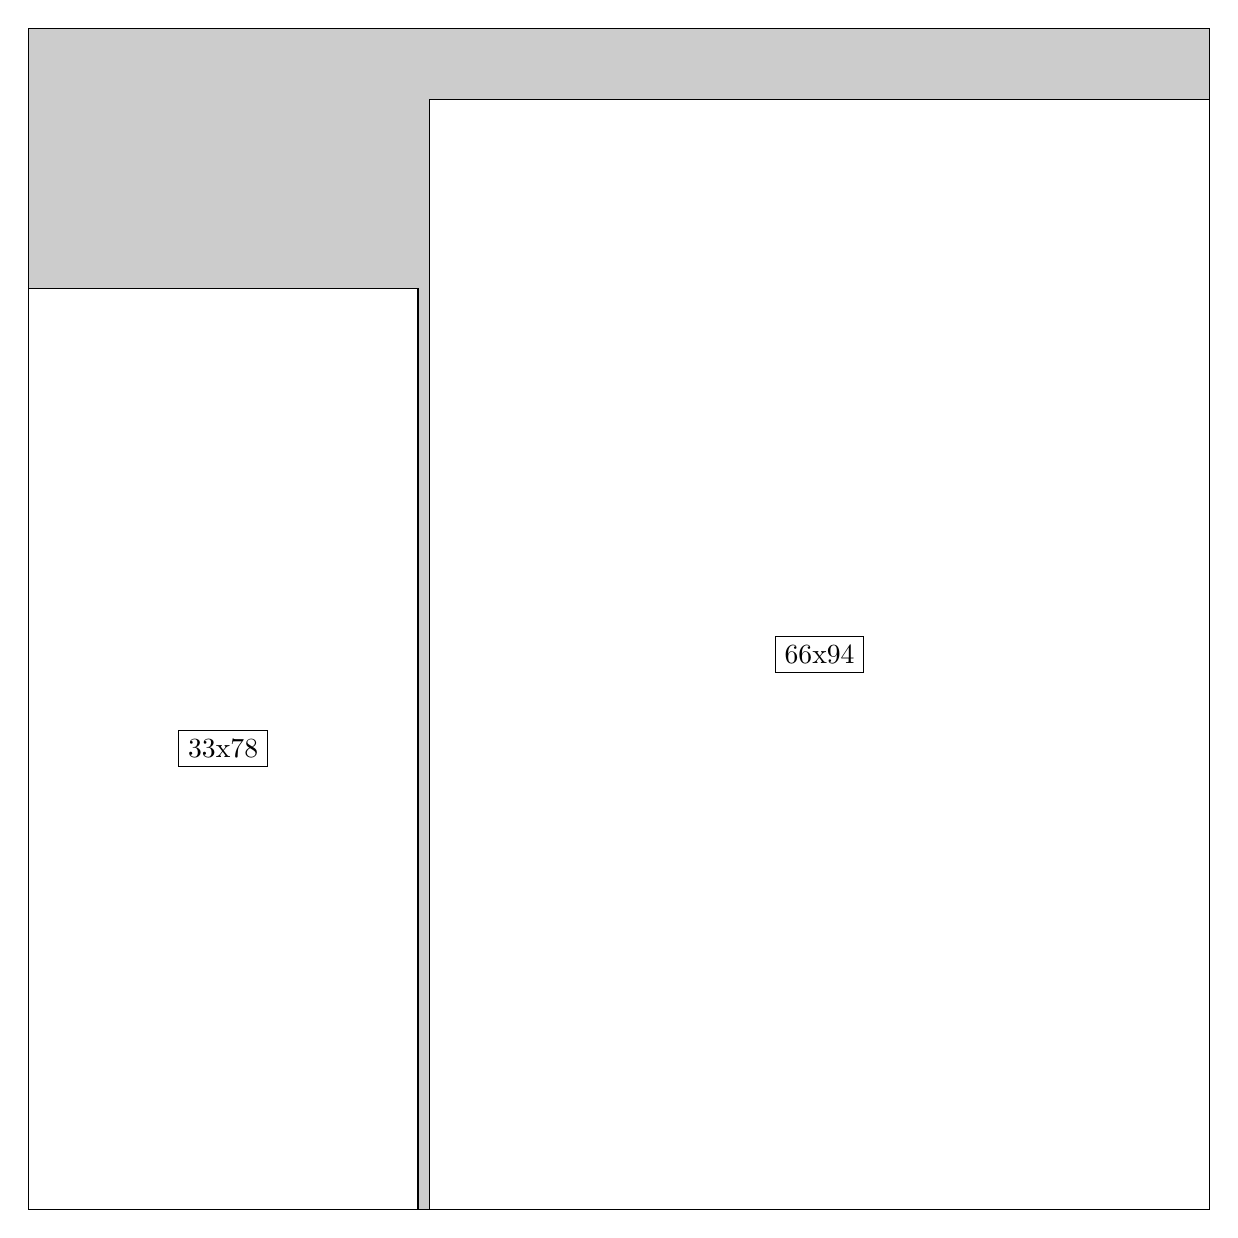
\begin{tikzpicture}[shorten >=1pt,scale=1.0,every node/.style={scale=1.0},->]
\tikzstyle{vertex}=[circle,fill=black!25,minimum size=14pt,inner sep=0pt]
\filldraw[fill=gray!40!white, draw=black] (0,0) rectangle (15.0,15.0);
\foreach \name/\x/\y/\w/\h in {66x94/5.1/0.0/9.9/14.1,33x78/0.0/0.0/4.95/11.7}
\filldraw[fill=white!40!white, draw=black] (\x,\y) rectangle node[draw] (\name) {\name} ++(\w,\h);
\end{tikzpicture}


w =66 , h =94 , x =34 , y =0 , v =6204
\par
w =33 , h =78 , x =0 , y =0 , v =2574
\par
\newpage


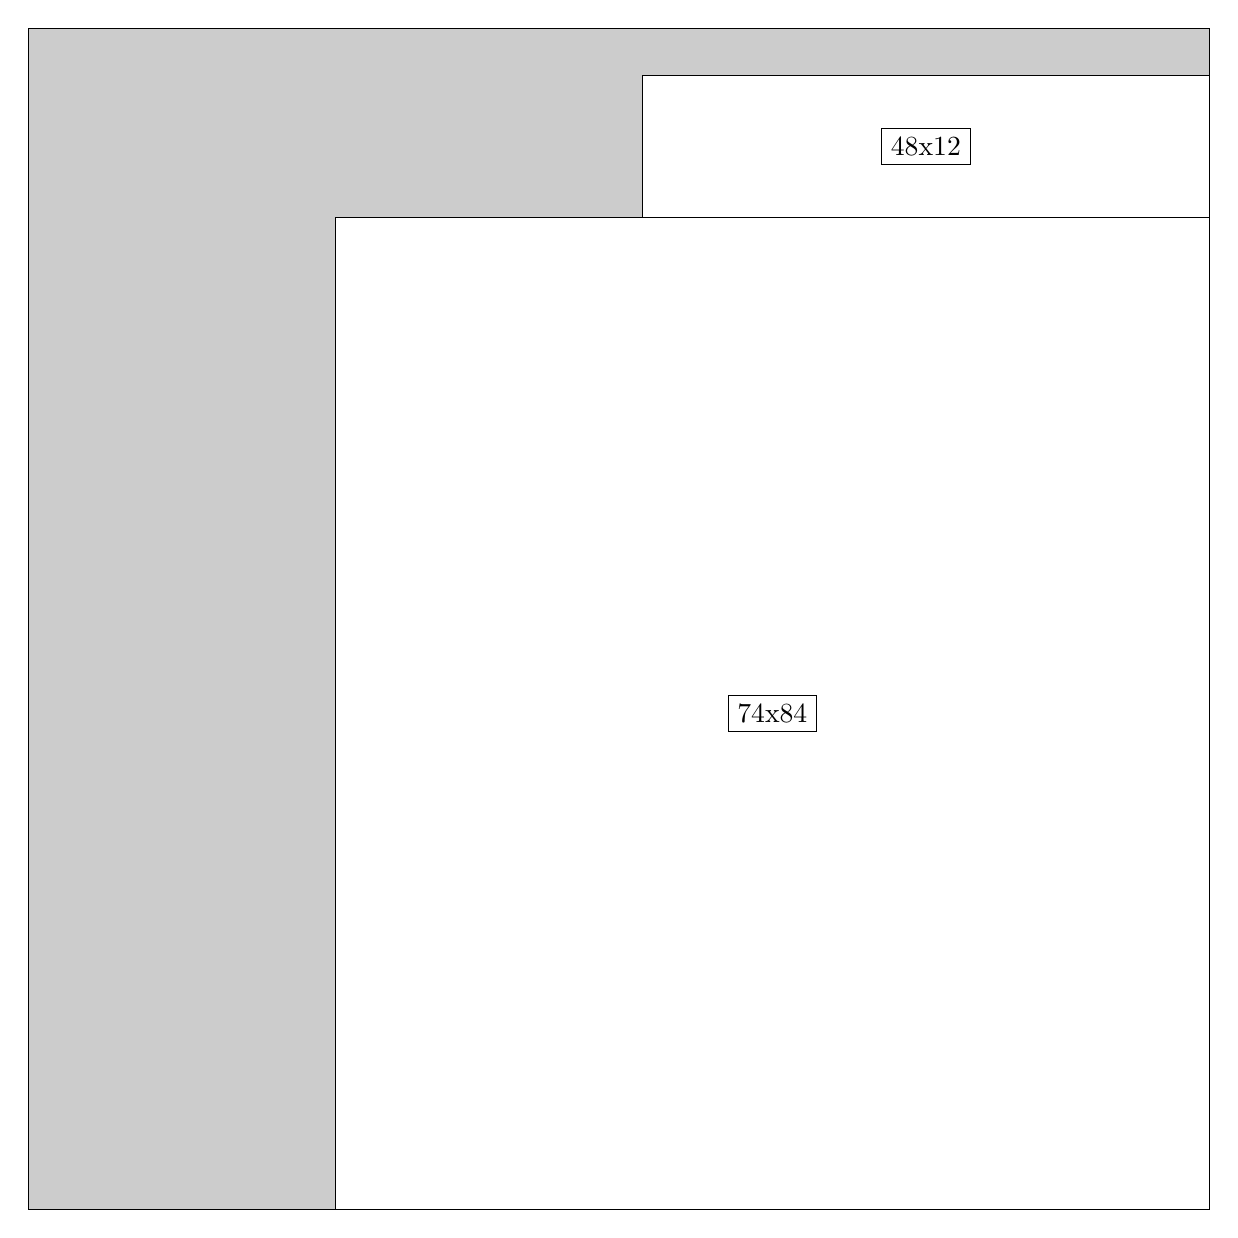
\begin{tikzpicture}[shorten >=1pt,scale=1.0,every node/.style={scale=1.0},->]
\tikzstyle{vertex}=[circle,fill=black!25,minimum size=14pt,inner sep=0pt]
\filldraw[fill=gray!40!white, draw=black] (0,0) rectangle (15.0,15.0);
\foreach \name/\x/\y/\w/\h in {74x84/3.9/0.0/11.1/12.6,48x12/7.8/12.6/7.199999999999999/1.7999999999999998}
\filldraw[fill=white!40!white, draw=black] (\x,\y) rectangle node[draw] (\name) {\name} ++(\w,\h);
\end{tikzpicture}


w =74 , h =84 , x =26 , y =0 , v =6216
\par
w =48 , h =12 , x =52 , y =84 , v =576
\par
\newpage



\begin{tikzpicture}[shorten >=1pt,scale=1.0,every node/.style={scale=1.0},->]
\tikzstyle{vertex}=[circle,fill=black!25,minimum size=14pt,inner sep=0pt]
\filldraw[fill=gray!40!white, draw=black] (0,0) rectangle (15.0,15.0);
\foreach \name/\x/\y/\w/\h in {73x98/4.05/0.0/10.95/14.7}
\filldraw[fill=white!40!white, draw=black] (\x,\y) rectangle node[draw] (\name) {\name} ++(\w,\h);
\end{tikzpicture}


w =73 , h =98 , x =27 , y =0 , v =7154
\par
\newpage


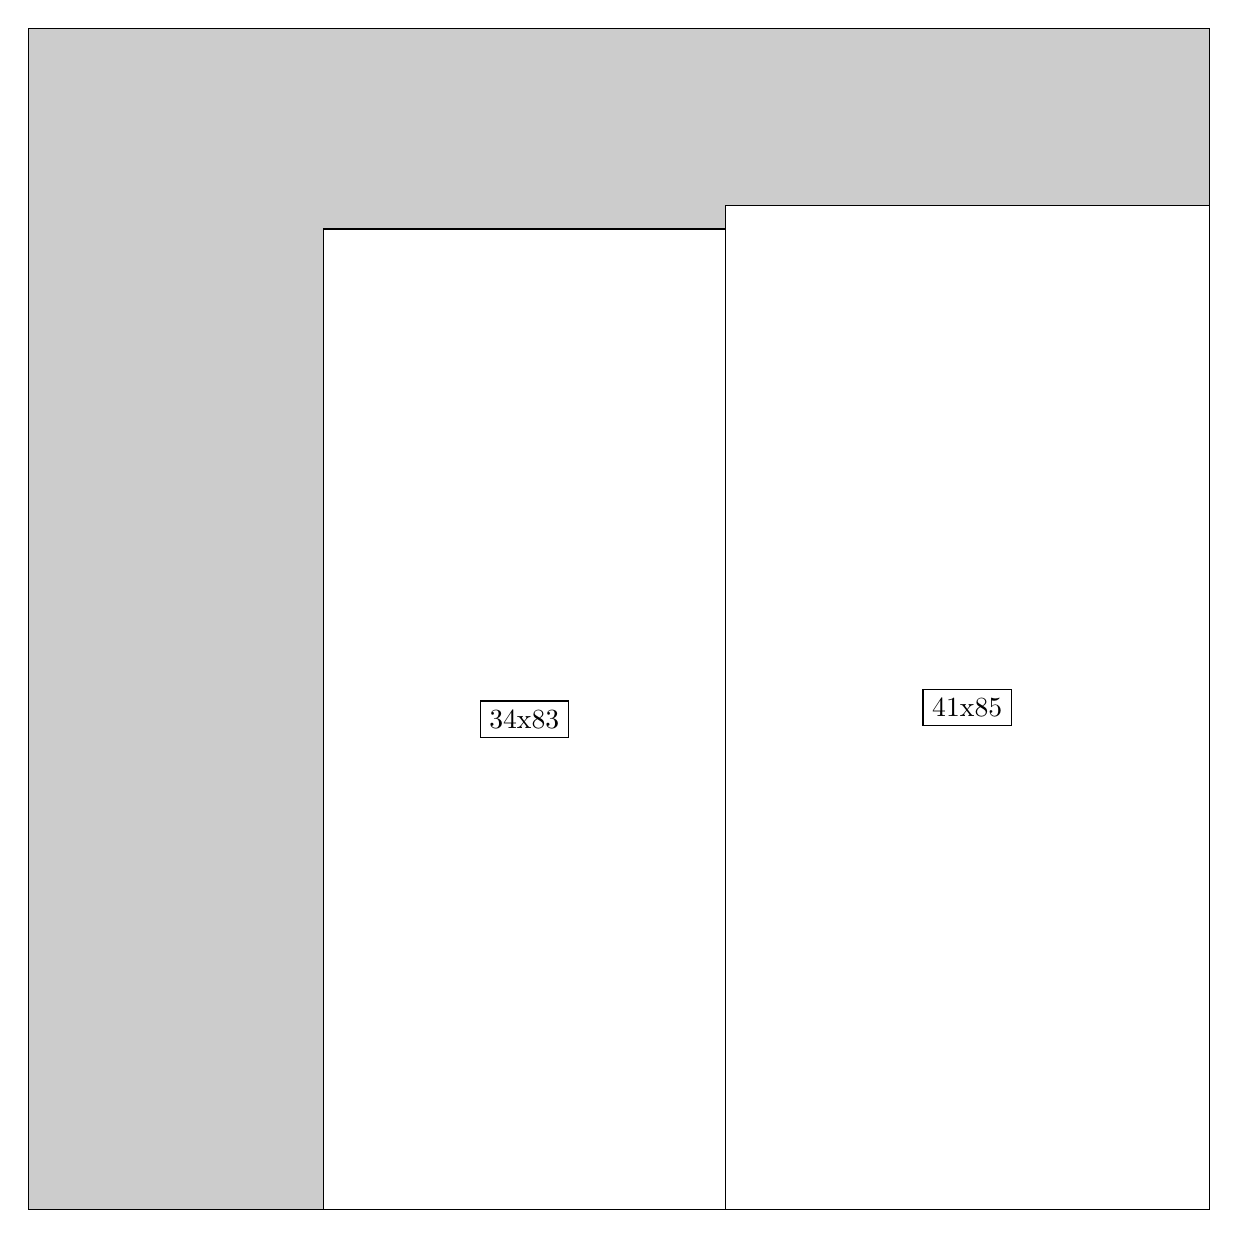
\begin{tikzpicture}[shorten >=1pt,scale=1.0,every node/.style={scale=1.0},->]
\tikzstyle{vertex}=[circle,fill=black!25,minimum size=14pt,inner sep=0pt]
\filldraw[fill=gray!40!white, draw=black] (0,0) rectangle (15.0,15.0);
\foreach \name/\x/\y/\w/\h in {41x85/8.85/0.0/6.1499999999999995/12.75,34x83/3.75/0.0/5.1/12.45}
\filldraw[fill=white!40!white, draw=black] (\x,\y) rectangle node[draw] (\name) {\name} ++(\w,\h);
\end{tikzpicture}


w =41 , h =85 , x =59 , y =0 , v =3485
\par
w =34 , h =83 , x =25 , y =0 , v =2822
\par
\newpage


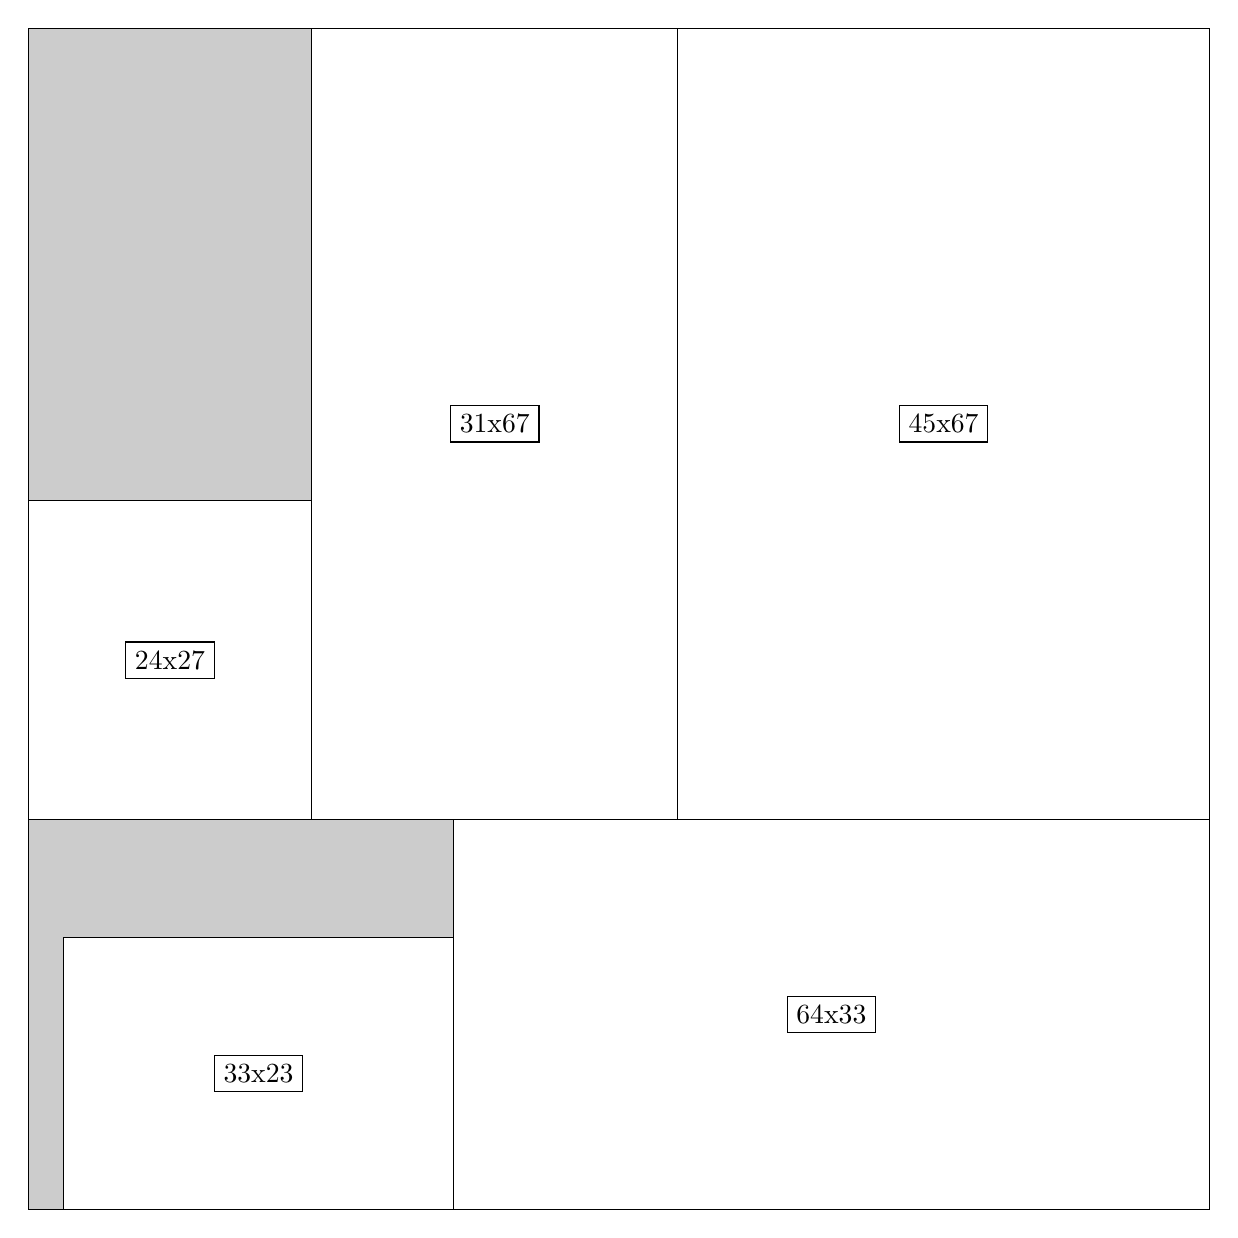
\begin{tikzpicture}[shorten >=1pt,scale=1.0,every node/.style={scale=1.0},->]
\tikzstyle{vertex}=[circle,fill=black!25,minimum size=14pt,inner sep=0pt]
\filldraw[fill=gray!40!white, draw=black] (0,0) rectangle (15.0,15.0);
\foreach \name/\x/\y/\w/\h in {64x33/5.3999999999999995/0.0/9.6/4.95,33x23/0.44999999999999996/0.0/4.95/3.4499999999999997,45x67/8.25/4.95/6.75/10.049999999999999,31x67/3.5999999999999996/4.95/4.6499999999999995/10.049999999999999,24x27/0.0/4.95/3.5999999999999996/4.05}
\filldraw[fill=white!40!white, draw=black] (\x,\y) rectangle node[draw] (\name) {\name} ++(\w,\h);
\end{tikzpicture}


w =64 , h =33 , x =36 , y =0 , v =2112
\par
w =33 , h =23 , x =3 , y =0 , v =759
\par
w =45 , h =67 , x =55 , y =33 , v =3015
\par
w =31 , h =67 , x =24 , y =33 , v =2077
\par
w =24 , h =27 , x =0 , y =33 , v =648
\par
\newpage


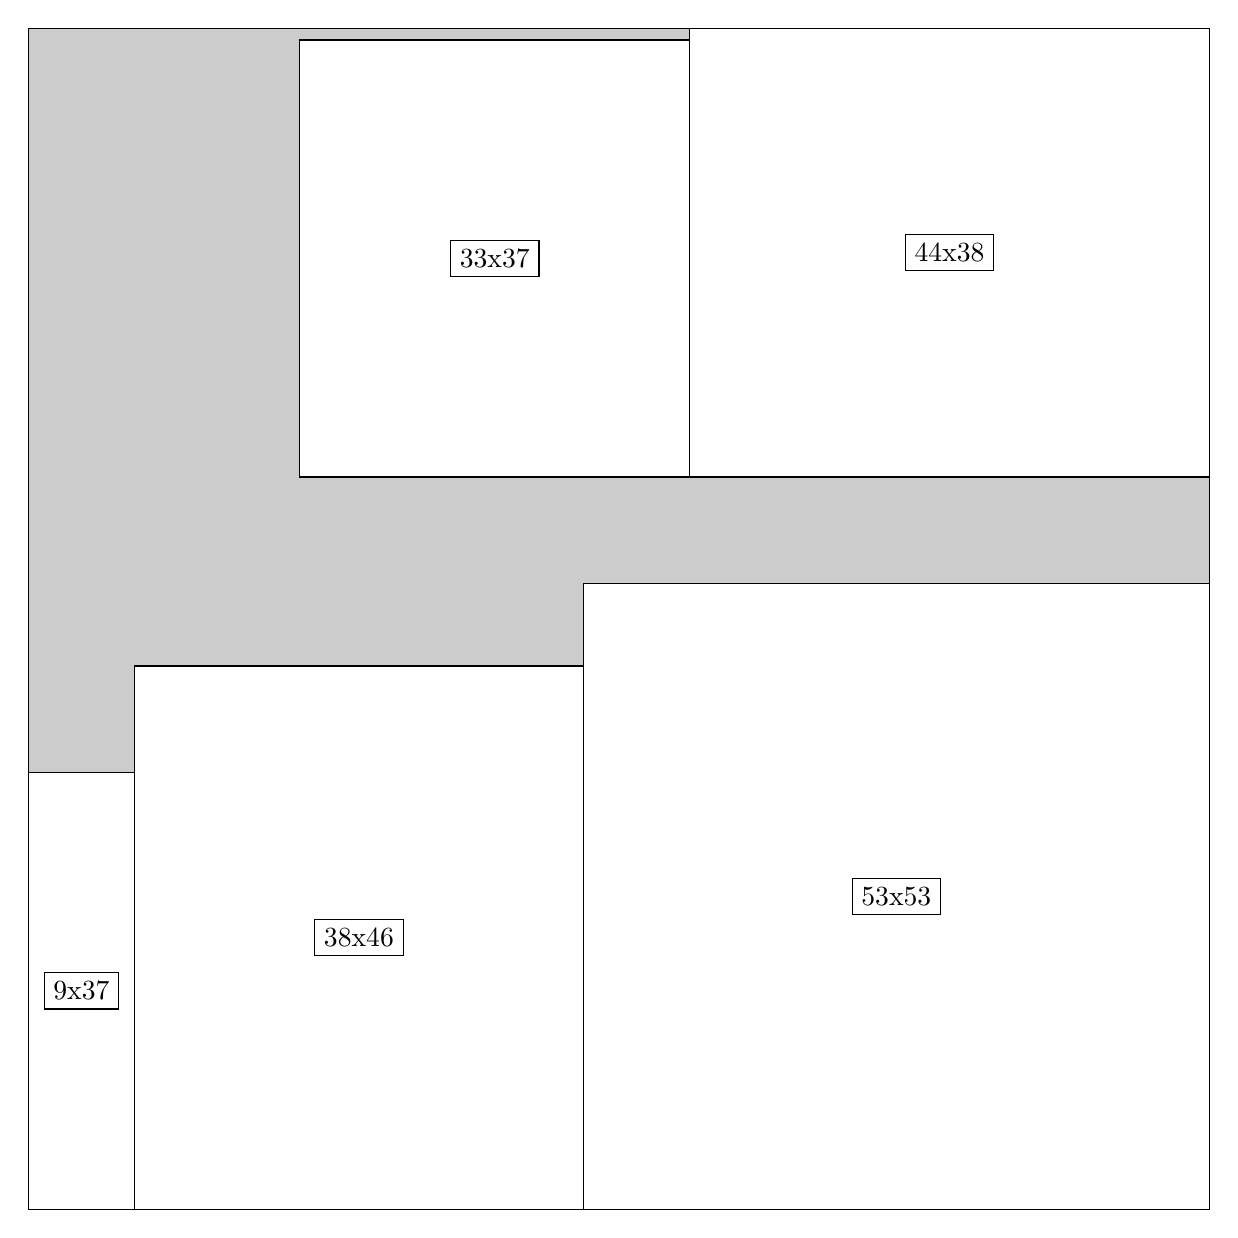
\begin{tikzpicture}[shorten >=1pt,scale=1.0,every node/.style={scale=1.0},->]
\tikzstyle{vertex}=[circle,fill=black!25,minimum size=14pt,inner sep=0pt]
\filldraw[fill=gray!40!white, draw=black] (0,0) rectangle (15.0,15.0);
\foreach \name/\x/\y/\w/\h in {53x53/7.05/0.0/7.949999999999999/7.949999999999999,38x46/1.3499999999999999/0.0/5.7/6.8999999999999995,9x37/0.0/0.0/1.3499999999999999/5.55,44x38/8.4/9.299999999999999/6.6/5.7,33x37/3.4499999999999997/9.299999999999999/4.95/5.55}
\filldraw[fill=white!40!white, draw=black] (\x,\y) rectangle node[draw] (\name) {\name} ++(\w,\h);
\end{tikzpicture}


w =53 , h =53 , x =47 , y =0 , v =2809
\par
w =38 , h =46 , x =9 , y =0 , v =1748
\par
w =9 , h =37 , x =0 , y =0 , v =333
\par
w =44 , h =38 , x =56 , y =62 , v =1672
\par
w =33 , h =37 , x =23 , y =62 , v =1221
\par
\newpage


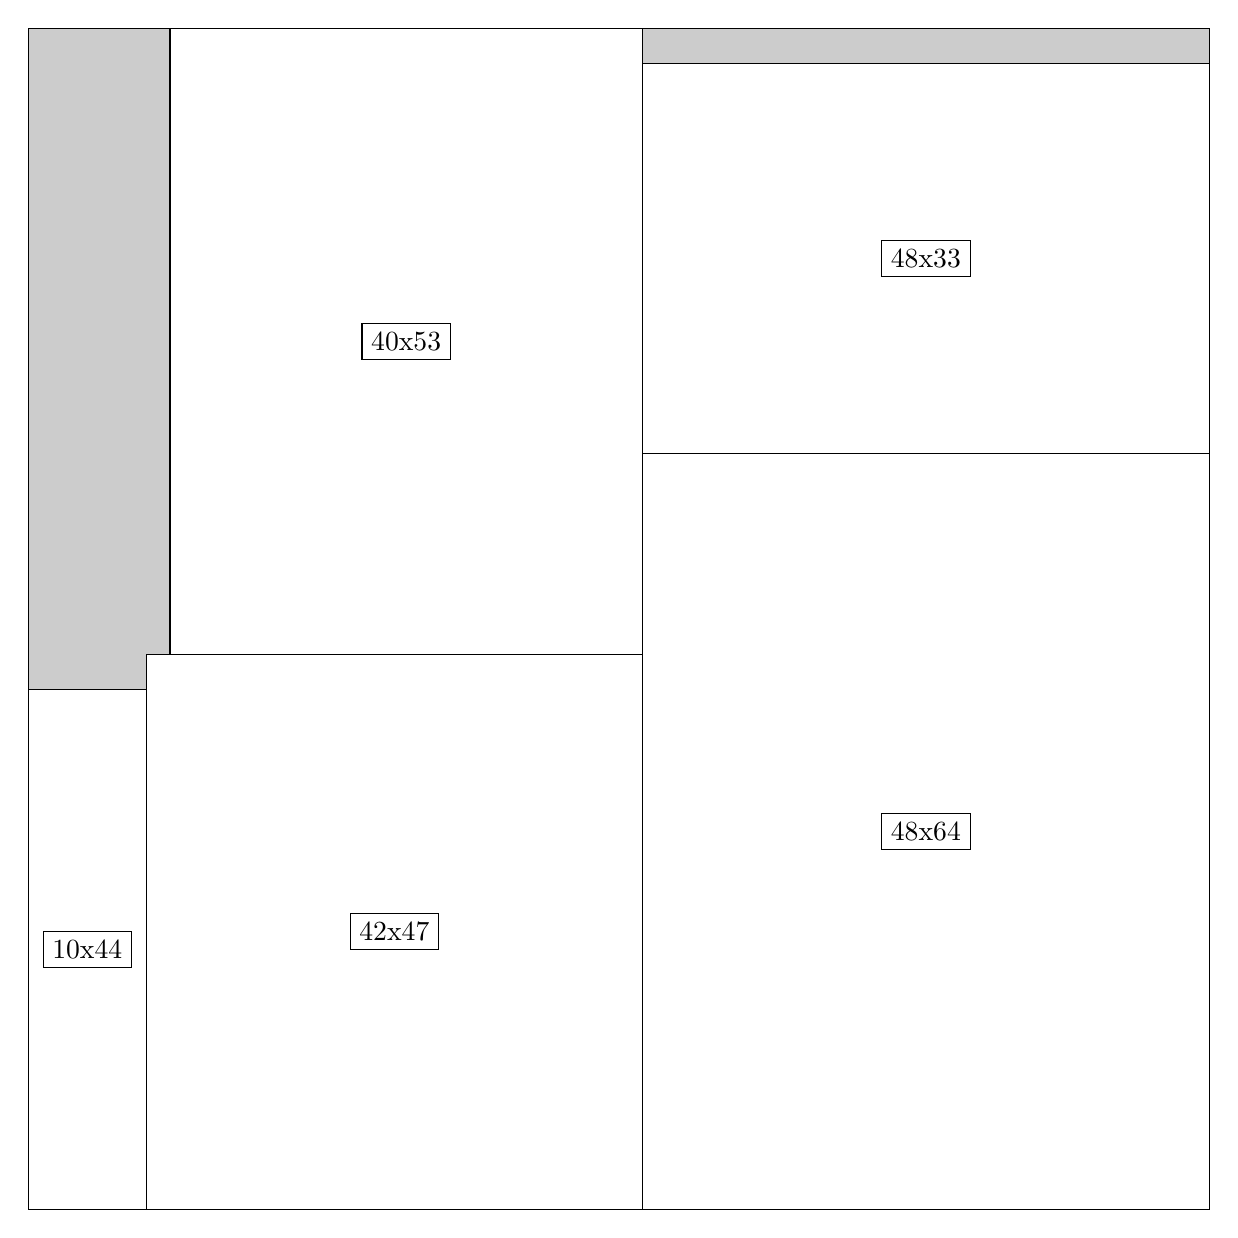
\begin{tikzpicture}[shorten >=1pt,scale=1.0,every node/.style={scale=1.0},->]
\tikzstyle{vertex}=[circle,fill=black!25,minimum size=14pt,inner sep=0pt]
\filldraw[fill=gray!40!white, draw=black] (0,0) rectangle (15.0,15.0);
\foreach \name/\x/\y/\w/\h in {48x64/7.8/0.0/7.199999999999999/9.6,48x33/7.8/9.6/7.199999999999999/4.95,42x47/1.5/0.0/6.3/7.05,10x44/0.0/0.0/1.5/6.6,40x53/1.7999999999999998/7.05/6.0/7.949999999999999}
\filldraw[fill=white!40!white, draw=black] (\x,\y) rectangle node[draw] (\name) {\name} ++(\w,\h);
\end{tikzpicture}


w =48 , h =64 , x =52 , y =0 , v =3072
\par
w =48 , h =33 , x =52 , y =64 , v =1584
\par
w =42 , h =47 , x =10 , y =0 , v =1974
\par
w =10 , h =44 , x =0 , y =0 , v =440
\par
w =40 , h =53 , x =12 , y =47 , v =2120
\par
\newpage


\end{document}